%----------------------------------------------------------------
%
%  File    :  survey-SVG.tex
%
%  Author  : Alexei Kruglov, TU Graz, Austria
% 
%  Created :  01 Dec 2016
% 
%  Changed :  06 Dec 2016
% 
%----------------------------------------------------------------


\section{Scalable Vector Graphics (SVG)}
\label{sect:SVG}
SVG (Scalable Vector Graphics) is an XML (Extensible Markup Language) based specification for describing two-dimensional graphics in a vector form. It is specified by W3C (World Wide Web Consortium). Initial release was made in 2001, and the latest release (1.1) was in 2011. Currently it is used in all latest major web browsers, such as Google Chrome, Mozilla Firefox and Internet Explorer, and in some vector graphics software editors, as Inkscape and Adobe Illustrator. In contrast to raster images, vector images are resolution independent, as the format itself is lossless. As mentioned before, the graphic is described in an XML textual file, which can be compressed with gzip. As a result of compression, web pages, where SVG is used load faster than those which use standard JPEG or PNG graphics solutions. Because graphics can be directly embedded into HTML, no extra HTTP requests are necessary. Above approaches lead to saving of the bandwidth, which is extremely important on the pages with higher loads. SVG has a support for different graphics effects and animations, which can be further enhanced with CSS and JavaScript. In case SVG graphic is made in a very complex node structure, browser can have problems rendering the image. In this case other technologies can be used. SVG integrates with other W3C standards such as the DOM and XSL. Since the graphics are described in vectors, we can change the properties of those through time to achieve much more complex animation than with just HTML elements \citep{w3schoolSVG}. 

\subsection{Defining Graphical Elementsin SVG} % (fold)
\label{sub:SVG_basic_elemnts}
As mentioned before SVG graphics can be embedded directly into HTML pages as an HTML element:

\begin{lstlisting}[
language=CSS,
label=list:BibACMIEEE,
caption={[Example of SVG Embedded Directyl into HTML]%
Simple example code one circle embedded directyl into HTML.
}
]
<html>
	<body>
		<svg width="100" height="100">
		  <circle cx="50" cy="50" r="40" stroke="green" stroke-width="4" fill="yellow" />
		</svg>
	</body>
</html>

\end{lstlisting}
\label{list:SVGHTML}
\begin{figure}[h]
\centering
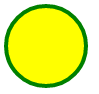
\includegraphics[keepaspectratio,scale=0.5]{images/circle.png}

\caption[SVG Basic Graphical Element]{
This example shows how simple to add one element (circle) embedded directyl into HTML. 
\imgcredit{Screenshot taken by the authors of this survey. The code behind the pages is by using the \citet{CircleHtml} online snippets as a base.}

}
\label{fig:circleHTML}
\end{figure}
SVG consists of different basic graphical elements, from which more complex elements can be derived. Basic elements included in SVG are:
\begin{description}
\item [<rect>]  is used to draw a rectangle and variations of the shape of a rectangle.
\item [<circle>] creates a simple circle with color options.
\item [<line>] draws a line.
\item [<polygon>] is used to create a graphic that contains at least three sides.
\item [<polyline>] provides any shape consisting of straight lines.
\item [<path>] defines a path. Use of a SVG editor is strongly encourage for path drawing to create complex graphics.
\end{description}

With these simple basic elements, one can build very complex shapes. With heli one has also additional graphics functions, where creation of a moving figure is also included. However, if these figures are created just by using SVG, the program code will be very large and difficult to read.
\begin{figure}[h]
\centering

\includegraphics[keepaspectratio,scale=0.5]{images/Car_svg.png}

\caption[Complex Image with Simple SVG Elements]{
Example to create one complex picture with simple SVG elements, with help geomety and color options.
\imgcredit{Screenshot taken by the authors of this survey. The code behind the pages is by using the \citet{CarSVG} online snippets as a base.}

}
\label{fig:Circle_HTML}
\end{figure}
% SVG basic graphical elements (end)
\subsection{Using SVG in CSS Animation } % (fold)
\label{sub:usingSVGanime}
SVG element is a specific DOM element, which includes himself syntax standard HTML-element. SVG elements have unique tags, attributes and behaviors that enable them to determine any form that offer the opportunity to essentially produce directly to the DOM, images, and thereby benefit from the JavaScript and CSS-based manipulation. There are three main advantages to create graphics in SVG comaped to statc images:
\begin{enumerate}
\item SVG can be compressed incredibly well. Certain images as SVGs are smaller than their PNG / JPEG equivalents.
\item SVG graphics can be scaled without any loss of clarity to any resolution. Therefore they look sharp on all desktop and mobile screens.
\item One can animate the individual components of the SVG graphic's performance with CSS or/and JavaScript. Keep in mind that SVG elements take some of the standard CSS properties, but not all.
\end{enumerate}

 In addition, SVG takes a certain set of "presentation" attributes, such as fill, x and y, which also serve to determine how the SVG is visually observed. There is no functional difference between the SVG specification of style using CSS, or as an SVG attribute \citep{w3schoolSVG}. In short, to animate and SVG, one has to:
\begin{enumerate}
\item Define the imeage as vectors in SVG.
\item Tranform the vectors with SVG, CSS or JavaScript.
\end{enumerate}
\begin{lstlisting}[
language=CSS,
label=list:BibACMIEEE,
caption={[SVG Declaration Example for Animation]%
SVG declaration example for animation.
}
]
<animateTransform attributeName="transform"
		attributeType="XML"
		type="translate"
		values="0 50;0 -50;"
		dur="2s"
		repeatCount="indefinite"/>

\end{lstlisting}
\label{list:animateTransorm}
%\subsubsection {Create SVG stucture into HTML} % (fold)


\begin{figure}[h]
\centering

\includegraphics[keepaspectratio,scale=0.5]{images/icon_svg.png}

\includegraphics[keepaspectratio,scale=0.5]{images/beer_svg.png}

\caption[SVG Animation Examples]{
Left example SVG is created by the authors to achieve a a trash bin animation with CSS. While the right example is a pure SVG beer animation. 
\imgcredit{Screenshots taken by the authors of this survey. The animation code behind the trash bin is done by the authors, while the SVG objects are provided by \citet{trashSVG}.The beer code is based on the \citet{beerSVG} online snippets as a base.}

}
\label{fig:SVGExamples}
\end{figure}


\begin{lstlisting}[
language=CSS,
label=list:BibACMIEEE,
caption={[Create SVG Stucture into HTML]%
The definition of the trash bin vectors, in figure \ref{fig:SVGExamples}, with the path element, proveded by \citet{trashSVG}.
}
]
<svg class="svg-icon" viewBox="0 0 20 20">
		<path id="svg-doc" d="M15.475,6.692l-4.084-4.083C11.32,
		2.538,11.223,2.5,11.125,2.5h-6c-0.413,0-0.75,0.337-0.75,
		0.75v13.5c0,0.412,0.337,0.75,0.75,0.75h9.75c0.412,
		0,0.75-0.338,0.75-0.75V6.94C15.609,6.839,15.554,6.771,
		15.475,6.692 M11.5,3.779l2.843,2.846H11.5V3.779z
		M14.875,16.75h-9.75V3.25h5.625V7c0,0.206,0.168,0.375,
		0.375,0.375h3.75V16.75z"
		transform="scale(0.25) translate(27.5)"></path>

		<path id="svg-bottom" fill="none" d="M16.471,
		5.962c-0.365-0.066-0.709,0.176-0.774,0.538l-1.843,
		10.217H6.096L4.255,6.5c-0.066-0.362-0.42-0.603-0.775-0.538
		C3.117,6.027,2.876,6.375,2.942,6.737l1.94,10.765c0.058,
		0.318,0.334,0.549,0.657,0.549h8.872c0.323,0,0.6-0.23,
		0.656-0.549l1.941-10.765C17.074,6.375,16.833,6.027,16.471,
		5.962z"
		transform="scale(0.75) translate(4,20)"></path>

		<path id="svg-deck" fill="none" d="M16.594,3.804H3.406
		c-0.369,0-0.667,0.298-0.667,0.667s0.299,0.667,0.667,
		0.667h13.188c0.369,0,0.667-0.298,0.667-0.667S16.963,
		3.804,16.594,3.804zM9.25,3.284h1.501c0.368,0,0.667-0.298,
		0.667-0.667c0-0.369-0.299-0.667-0.667-0.667H9.25c-0.369,
		0-0.667,0.298-0.667,0.667C8.583,2.985,8.882,3.284,9.25,3.284z"
		transform="scale(0.75) translate(4,20)"></path>
	</svg>

\end{lstlisting}
\label{list:SVGStuctureHTML}

% \subsubsection {Define keyframe in CSS} % (fold)
\begin{lstlisting}[
language=CSS,
label=list:BibACMIEEE,
caption={[SVG Animation with CSS Declaration]%
The animation of the trash bin vectors, in figure \ref{fig:SVGExamples}, with the path element, proveded by \citet{trashSVG}. The animation wokrs together with the vectors in the previous listing.
}
]
#svg-doc{
	fill:red;
	animation: doc-delete 4s linear infinite;
}

#svg-deck{
	transform-origin: 100% 50%;
	animation: deck-rot 4s linear infinite;
}

@keyframes doc-delete {
	0% { transform: translate(75%) scale(0.25); }
	15% { transform: translate(75%) scale(0.25); }
	65% { transform: translate(85%,150%) scale(0.1) rotate(-180deg);}
	100% { transform: translate(85%,150%) scale(0.1); opacity: 0;}
}

@keyframes deck-rot {
	0% { transform: translate(-9%, 440%) rotate(0deg) scale(0.75); }
	25% { transform: translate(-9%, 440%) rotate(90deg) scale(0.75);}
	40% { transform: translate(-9%, 440%) rotate(90deg) scale(0.75);}
	65% { transform: translate(-9%, 440%) rotate(0deg) scale(0.75);}
	100% { transform: translate(-9%, 440%) rotate(0deg) scale(0.75);}

\end{lstlisting}
\label{list:Keys_CSS}